\documentclass[12pt,a4paper]{article}

%% ============================================================
%%  PREAMBLE
%% ============================================================
\usepackage{amsmath}
\usepackage{amssymb}
\usepackage{geometry}
\geometry{margin=2.5cm}
\usepackage{booktabs}
\usepackage{xcolor}
\usepackage{hyperref}
\usepackage{listings}
\usepackage{pgfplots}
\pgfplotsset{compat=1.18}
\usepackage{tcolorbox}
\tcbuselibrary{skins, breakable}
\usepackage{enumitem}
\usepackage{fancyhdr}
\usepackage{tikz}
\usepackage{array}
\usepackage{subcaption}

%% ---- tcolorbox environments (positional title [1]) ----------
\newtcolorbox{curiositybox}[1]{colback=yellow!10, colframe=orange!80!black, fonttitle=\bfseries, title=#1, breakable}
\newtcolorbox{infobox}[1]{colback=blue!5, colframe=blue!60!black, fonttitle=\bfseries, title=#1, breakable}
\newtcolorbox{mistakebox}[1]{colback=red!5, colframe=red!60!black, fonttitle=\bfseries, title=#1, breakable}
\newtcolorbox{learnbox}[1]{colback=green!5, colframe=green!60!black, fonttitle=\bfseries, title=#1, breakable}

%% ---- lstlisting for Python ---------------------------------
\lstset{language=Python,
        basicstyle=\ttfamily\small,
        keywordstyle=\color{blue},
        commentstyle=\color{gray},
        stringstyle=\color{orange},
        showstringspaces=false,
        numbers=left,
        numberstyle=\tiny,
        breaklines=true,
        frame=single}

%% ---- fancyhdr ----------------------------------------------
\pagestyle{fancy}
\fancyhf{}
\lhead{Topic 08: Convolution Theorem (FT)}
\rhead{Unit V --- Fourier Series \& Transforms}
\cfoot{\thepage}

%% ---- Title -------------------------------------------------
\title{Topic 08: Convolution Theorem for Fourier Transforms \\
       \large Unit V --- Fourier Series \& Fourier Transforms}
\author{23A54201 --- Mathematics IV (Transform Techniques)\\
        JNTUA College of Engineering (Autonomous)}
\date{}

%% ============================================================
\begin{document}
\maketitle
\tableofcontents
\newpage

%% ============================================================
\section{Opening Hook}
%% ============================================================

\begin{curiositybox}{Hook}
An audio engineer wants to add studio-quality reverb to a dry vocal recording.
Doing this directly means sliding the recording against a ``room response'' signal
and summing overlapping products at every time shift --- a slow, expensive operation
called convolution. But there is a shortcut: transform both signals into the frequency
domain, multiply them point-by-point (instant), and transform back. This one shortcut
--- the Convolution Theorem --- is why every digital reverb, equalizer, and
image-blur filter on your phone runs in real time instead of taking minutes.
\end{curiositybox}

%% ============================================================
\section{Why This Topic Exists}
%% ============================================================

Before we begin, here is the honest answer to why you are reading this.
Convolution is the mathematical operation that describes how one signal modifies
another --- it underlies everything from echo and reverb to image sharpening and
noise filtering. Performing convolution directly requires evaluating an integral
(or sum) whose cost grows quadratically with signal length.
Moving to the frequency domain converts that expensive integral into an
instantaneous pointwise multiplication, cutting cost from $O(n^2)$ to $O(n\log n)$
via the Fast Fourier Transform. \emph{That} is why engineers bother learning Fourier
transforms at all.

\begin{center}
\begin{tabular}{>{\bfseries}p{6cm} p{8cm}}
\toprule
Common Mistake & Consequence \\
\midrule
Confusing Fourier convolution with Laplace convolution &
  Using the one-sided $[0,\infty)$ formula for a problem defined on $(-\infty,\infty)$,
  giving a wrong or undefined result \\[4pt]
Forgetting the $\sqrt{2\pi}$ or $2\pi$ normalisation factor &
  Getting an answer off by a constant multiple \\[4pt]
Treating convolution as ordinary multiplication of functions &
  Computing $f(t)g(t)$ instead of the sliding integral
  $\int f(\tau)g(t-\tau)\,d\tau$ \\
\bottomrule
\end{tabular}
\end{center}

\begin{learnbox}{Key Takeaway}
The Convolution Theorem is the single biggest reason engineers use the Fourier
transform: convolution in time $\longleftrightarrow$ multiplication in frequency.
\end{learnbox}

%% ============================================================
\section{You Already Know This (Intuition First)}
%% ============================================================

Imagine two ink drops placed in still water. Each drop spreads outward in a smooth
circular wave. The resulting shade at any point is a weighted sum of all the ways
the two spreading influences overlap as time passes. This is convolution: at each
instant $t$, slide one signal past the other, multiply overlapping values, and add
them up.

You have already seen this idea in the Laplace Convolution Theorem (Unit IV,
Topic~07): the hard integral $\int_0^t f(\tau)g(t-\tau)\,d\tau$ became simple
multiplication $F(s)\cdot G(s)$ in the s-domain. The Fourier Convolution Theorem
is the same story --- but now for two-sided, non-causal signals defined on
$(-\infty,\infty)$. The limits of integration change, but the core idea is
identical: a hard time-domain integral becomes an effortless frequency-domain
multiplication.

%% ============================================================
\section{Definition: Convolution of Two Functions}
%% ============================================================

\begin{infobox}{Convolution of Two Functions}
\textbf{Definition.} Let $f$ and $g$ be functions defined on $(-\infty,\infty)$.
Their \emph{convolution} $(f*g)(t)$ is defined by
\[
  (f * g)(t) \;=\; \int_{-\infty}^{\infty} f(\tau)\,g(t-\tau)\,d\tau,
\]
provided the integral converges absolutely.

\medskip
\textbf{Geometric Interpretation (flip-and-slide).}
\begin{enumerate}[label=\arabic*.]
  \item \textbf{Flip:} Reflect $g$ about the vertical axis to get $g(-\tau)$.
  \item \textbf{Slide:} Shift the flipped version by $t$ to get $g(t-\tau)$.
  \item \textbf{Multiply:} Form the product $f(\tau)\cdot g(t-\tau)$.
  \item \textbf{Integrate:} Sum (integrate) over all $\tau$ to get the single
        number $(f*g)(t)$.
  \item \textbf{Repeat} for every value of $t$ to trace out the full convolution.
\end{enumerate}

\medskip
\textbf{Properties.}
\begin{itemize}
  \item \emph{Commutative:} $f*g = g*f$
  \item \emph{Associative:} $(f*g)*h = f*(g*h)$
  \item \emph{Distributive:} $f*(g+h) = f*g + f*h$
\end{itemize}

\medskip
\textbf{Contrast with Laplace Convolution.}
\begin{center}
\begin{tabular}{lll}
\toprule
Feature & Fourier Convolution & Laplace Convolution \\
\midrule
Integration limits & $-\infty$ to $\infty$ & $0$ to $t$ \\
Signal type & Two-sided, non-causal & Causal ($f,g=0$ for $t<0$) \\
Domain & $\omega$-domain & $s$-domain \\
Normalisation & May carry $2\pi$ factor & No extra factor \\
\bottomrule
\end{tabular}
\end{center}
\end{infobox}

%% ============================================================
\section{Statement of the Convolution Theorem}
%% ============================================================

\begin{infobox}{Convolution Theorem for Fourier Transforms}
\textbf{Theorem (Convolution in Time, Multiplication in Frequency).}
If $\mathcal{F}\{f(t)\} = F(\omega)$ and $\mathcal{F}\{g(t)\} = G(\omega)$, then
\[
  \boxed{\mathcal{F}\{(f*g)(t)\}(\omega) \;=\; F(\omega)\cdot G(\omega)}
\]

\medskip
\textbf{Dual Theorem (Multiplication in Time, Convolution in Frequency).}
\[
  \boxed{\mathcal{F}\{f(t)\cdot g(t)\}(\omega) \;=\; \frac{1}{2\pi}\,(F*G)(\omega)}
\]
where $(F*G)(\omega) = \int_{-\infty}^{\infty}F(\xi)\,G(\omega-\xi)\,d\xi$.

\medskip
\textbf{Normalisation Convention Note.}
The constant $\frac{1}{2\pi}$ appears here because we use the asymmetric convention
\[
  \mathcal{F}\{f(t)\}(\omega) = \int_{-\infty}^{\infty} f(t)\,e^{-i\omega t}\,dt,
  \qquad
  f(t) = \frac{1}{2\pi}\int_{-\infty}^{\infty}F(\omega)\,e^{i\omega t}\,d\omega.
\]
If the symmetric convention $\frac{1}{\sqrt{2\pi}}$ is used for both transform and
inverse, the dual theorem carries $\frac{1}{\sqrt{2\pi}}$ instead. Always check
which convention your reference uses before applying the theorem.
\end{infobox}

%% ============================================================
\section{Proof of the Convolution Theorem}
%% ============================================================

\begin{infobox}{Full Proof of the Convolution Theorem}
\textbf{Claim:} $\mathcal{F}\{(f*g)(t)\}(\omega) = F(\omega)\cdot G(\omega)$.

\medskip
\textbf{Step 1.} Write the Fourier transform of the convolution directly:
\[
  \mathcal{F}\{(f*g)\}(\omega)
  = \int_{-\infty}^{\infty}
      \left[\int_{-\infty}^{\infty} f(\tau)\,g(t-\tau)\,d\tau\right]
    e^{-i\omega t}\,dt.
\]

\textbf{Step 2.} Swap the order of integration (justified by Fubini's theorem,
valid when $f,g \in L^1(\mathbb{R})$, i.e., both are absolutely integrable):
\[
  = \int_{-\infty}^{\infty} f(\tau)
      \left[\int_{-\infty}^{\infty} g(t-\tau)\,e^{-i\omega t}\,dt\right]
    d\tau.
\]

\textbf{Step 3.} In the inner integral, substitute $u = t - \tau$, so $t = u+\tau$,
$dt = du$, and the limits remain $-\infty$ to $\infty$:
\[
  \int_{-\infty}^{\infty} g(t-\tau)\,e^{-i\omega t}\,dt
  = \int_{-\infty}^{\infty} g(u)\,e^{-i\omega(u+\tau)}\,du
  = e^{-i\omega\tau}\int_{-\infty}^{\infty} g(u)\,e^{-i\omega u}\,du
  = e^{-i\omega\tau}\,G(\omega).
\]

\textbf{Step 4.} Substitute back:
\[
  \mathcal{F}\{f*g\}(\omega)
  = \int_{-\infty}^{\infty} f(\tau)\,e^{-i\omega\tau}\,G(\omega)\,d\tau
  = G(\omega)\int_{-\infty}^{\infty} f(\tau)\,e^{-i\omega\tau}\,d\tau
  = G(\omega)\,F(\omega).
\]

\textbf{Conclusion:}
\[
  \mathcal{F}\{(f*g)(t)\}(\omega) = F(\omega)\cdot G(\omega). \qquad \square
\]
\end{infobox}

%% ============================================================
\section{Convolution Theorem for Fourier Sine and Cosine Transforms}
%% ============================================================

\begin{infobox}{Sine and Cosine Transform Convolution Results}
For functions defined on $[0,\infty)$, the Fourier sine and cosine transforms have
analogous (but more intricate) convolution-type identities. These use special
``cosine/sine convolutions'' rather than the standard two-sided convolution.

\medskip
\begin{center}
\begin{tabular}{>{\bfseries}p{3.5cm} p{5.5cm} p{5.5cm}}
\toprule
Transform Type & Convolution Definition & Theorem Statement \\
\midrule
Fourier Cosine ($F_c$) &
  $\displaystyle (f \stackrel{c}{*} g)(t) = \int_0^\infty f(\tau)
  \bigl[g(|t-\tau|)+g(t+\tau)\bigr]\,d\tau$ &
  $F_c\{f \stackrel{c}{*} g\}(\omega) = F_c(\omega)\cdot G_c(\omega)$ \\[10pt]
Fourier Sine ($F_s$) &
  $\displaystyle (f \stackrel{s}{*} g)(t) = \int_0^\infty f(\tau)
  \bigl[g(|t-\tau|)-g(t+\tau)\bigr]\,d\tau$ &
  $F_s\{f \stackrel{s}{*} g\}(\omega) = F_s(\omega)\cdot G_c(\omega)$ \\[10pt]
Mixed ($F_s$, $F_c$) &
  Combines sine and cosine transforms &
  $F_c\{f \stackrel{s}{*} g\}(\omega) = F_s(\omega)\cdot G_s(\omega)$ \\
\bottomrule
\end{tabular}
\end{center}

\medskip
\textbf{Note:} In practice, engineering students primarily use the full Fourier
convolution theorem. The sine/cosine variants arise mainly in problems with
half-line symmetry (e.g., heat equation on a semi-infinite rod).
\end{infobox}

%% ============================================================
\section{Why This Matters: Filtering and Systems}
%% ============================================================

\begin{infobox}{Linear Time-Invariant (LTI) Systems and the Convolution Theorem}
\textbf{Setup.} A Linear Time-Invariant (LTI) system with impulse response $h(t)$
produces output $y(t)$ for input $x(t)$ via:
\[
  y(t) = (h * x)(t) = \int_{-\infty}^{\infty} h(\tau)\,x(t-\tau)\,d\tau.
\]

\textbf{In the frequency domain:} By the Convolution Theorem,
\[
  \boxed{Y(\omega) = H(\omega)\cdot X(\omega)}
\]
where $H(\omega) = \mathcal{F}\{h(t)\}$ is called the \emph{transfer function}
(or frequency response) of the system.

\medskip
\textbf{Block Diagram View.}

\begin{center}
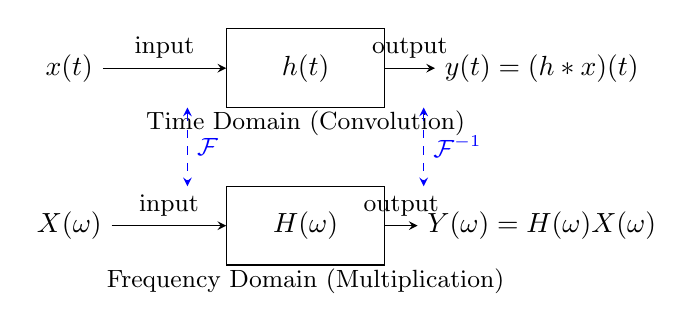
\begin{tikzpicture}[>=stealth, node distance=3.5cm]
  % Time domain
  \node (xt) at (0,1) {$x(t)$};
  \node[draw, rectangle, minimum width=2cm, minimum height=1cm] (sys_t) at (3,1) {$h(t)$};
  \node (yt) at (6,1) {$y(t) = (h*x)(t)$};
  \draw[->] (xt) -- (sys_t) node[midway, above] {\small input};
  \draw[->] (sys_t) -- (yt) node[midway, above] {\small output};
  \node at (3, 0.3) {\small Time Domain (Convolution)};

  % Frequency domain
  \node (xw) at (0,-1) {$X(\omega)$};
  \node[draw, rectangle, minimum width=2cm, minimum height=1cm] (sys_w) at (3,-1) {$H(\omega)$};
  \node (yw) at (6,-1) {$Y(\omega) = H(\omega)X(\omega)$};
  \draw[->] (xw) -- (sys_w) node[midway, above] {\small input};
  \draw[->] (sys_w) -- (yw) node[midway, above] {\small output};
  \node at (3, -1.7) {\small Frequency Domain (Multiplication)};

  % Connecting arrows
  \draw[<->, dashed, blue] (1.5,0.5) -- (1.5,-0.5) node[midway, right] {\small $\mathcal{F}$};
  \draw[<->, dashed, blue] (4.5,0.5) -- (4.5,-0.5) node[midway, right] {\small $\mathcal{F}^{-1}$};
\end{tikzpicture}
\end{center}

\medskip
\textbf{Physical meaning.} $H(\omega)$ is the system's ``personality'' in
frequency: it boosts or attenuates each frequency component of the input.
A low-pass filter, for example, has $|H(\omega)| \approx 1$ for low $\omega$
and $|H(\omega)| \approx 0$ for high $\omega$. By designing $H(\omega)$ in the
frequency domain (easy), you automatically determine the time-domain
filtering operation (convolution with $h(t)$) --- without ever computing an
integral directly.
\end{infobox}

%% ============================================================
\section{Visualising Convolution}
%% ============================================================

The figure below shows two rectangular pulse functions $f(t)$ and $g(t)$ (each
of width~2, height~1, centred at~0) and their convolution $(f*g)(t)$, which is
the well-known triangular pulse of width~4 and peak value~2.

\begin{center}
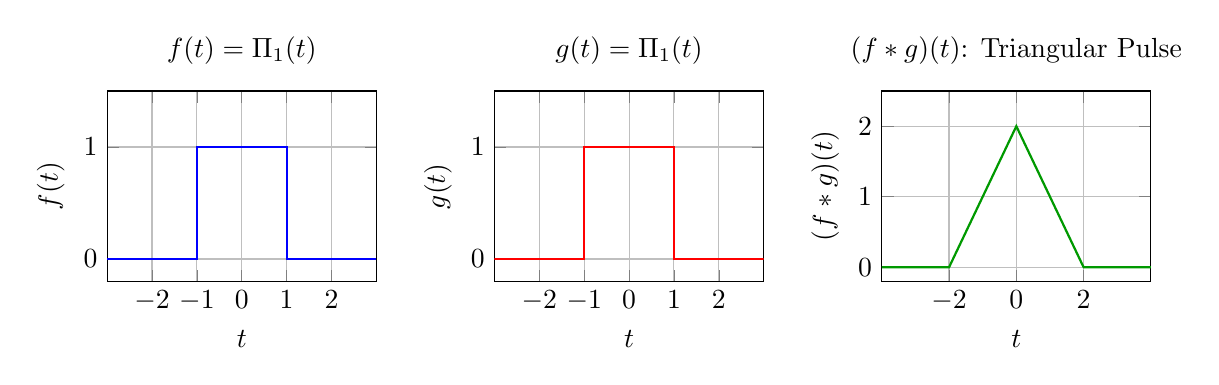
\begin{tikzpicture}
\begin{axis}[
  name=ax1,
  width=5cm, height=4cm,
  xlabel={$t$}, ylabel={$f(t)$},
  xmin=-3, xmax=3,
  ymin=-0.2, ymax=1.5,
  grid=major,
  title={$f(t) = \Pi_1(t)$},
  xtick={-2,-1,0,1,2},
  ytick={0,1},
]
\addplot[blue, thick] coordinates {(-3,0)(-1,0)(-1,1)(1,1)(1,0)(3,0)};
\end{axis}

\begin{axis}[
  name=ax2,
  at={(ax1.east)}, anchor=west, xshift=1.5cm,
  width=5cm, height=4cm,
  xlabel={$t$}, ylabel={$g(t)$},
  xmin=-3, xmax=3,
  ymin=-0.2, ymax=1.5,
  grid=major,
  title={$g(t) = \Pi_1(t)$},
  xtick={-2,-1,0,1,2},
  ytick={0,1},
]
\addplot[red, thick] coordinates {(-3,0)(-1,0)(-1,1)(1,1)(1,0)(3,0)};
\end{axis}

\begin{axis}[
  name=ax3,
  at={(ax2.east)}, anchor=west, xshift=1.5cm,
  width=5cm, height=4cm,
  xlabel={$t$}, ylabel={$(f*g)(t)$},
  xmin=-4, xmax=4,
  ymin=-0.2, ymax=2.5,
  grid=major,
  title={$(f*g)(t)$: Triangular Pulse},
  xtick={-2,0,2},
  ytick={0,1,2},
]
\addplot[green!60!black, thick] coordinates {(-4,0)(-2,0)(0,2)(2,0)(4,0)};
\end{axis}
\end{tikzpicture}
\end{center}

The convolution ``smears'' or ``blurs'' the signal: two sharp rectangular pulses
combine into a smooth triangular pulse. This smearing effect is why convolution
models physical processes like diffusion, reverb, and optical blurring --- each is
a system ``spreading'' a point stimulus into a broader response.

%% ============================================================
\section{Worked Examples}
%% ============================================================

\begin{infobox}{Example 1: Convolution Theorem for Double-Sided Exponentials}
\textbf{Problem.} Let $f(t) = e^{-a|t|}$ and $g(t) = e^{-b|t|}$ with $a,b>0$,
$a \neq b$. Verify the Convolution Theorem by computing $F(\omega)$ and $G(\omega)$
independently, then multiplying.

\medskip
\textbf{Step 1.} Recall from the standard Fourier transform table (Topic~07) that
for $\alpha > 0$:
\[
  \mathcal{F}\left\{e^{-\alpha|t|}\right\}(\omega)
  = \frac{2\alpha}{\alpha^2 + \omega^2}.
\]

\textbf{Step 2.} Apply this formula:
\[
  F(\omega) = \mathcal{F}\left\{e^{-a|t|}\right\}(\omega) = \frac{2a}{a^2+\omega^2},
  \qquad
  G(\omega) = \mathcal{F}\left\{e^{-b|t|}\right\}(\omega) = \frac{2b}{b^2+\omega^2}.
\]

\textbf{Step 3.} By the Convolution Theorem:
\[
  \mathcal{F}\{(f*g)(t)\}(\omega) = F(\omega)\cdot G(\omega)
  = \frac{2a}{a^2+\omega^2} \cdot \frac{2b}{b^2+\omega^2}
  = \frac{4ab}{(a^2+\omega^2)(b^2+\omega^2)}.
\]

\textbf{Step 4.} Use partial fractions to confirm this is itself a recognisable
Fourier transform. Write:
\[
  \frac{4ab}{(a^2+\omega^2)(b^2+\omega^2)}
  = \frac{4ab}{b^2-a^2}\left(\frac{1}{a^2+\omega^2} - \frac{1}{b^2+\omega^2}\right)
  \quad (a \neq b).
\]
Taking the inverse Fourier transform:
\[
  (f*g)(t) = \frac{4ab}{b^2-a^2}\left(\frac{1}{2a}e^{-a|t|} - \frac{1}{2b}e^{-b|t|}\right)
  = \frac{2b}{b^2-a^2}\,e^{-a|t|} - \frac{2a}{b^2-a^2}\,e^{-b|t|}.
\]

\textbf{Conclusion.} The theorem has been verified: multiplying $F(\omega)$ by
$G(\omega)$ gives exactly the Fourier transform of the convolution $(f*g)(t)$.
\end{infobox}

\begin{learnbox}{What Did We Learn? (Example 1)}
For double-sided exponential decays $e^{-a|t|}$, the Fourier transform is the
familiar Lorentzian $\frac{2a}{a^2+\omega^2}$. The Convolution Theorem converts
the convolution integral into a product of two such Lorentzians, and partial
fractions recovers the time-domain answer without ever evaluating the integral.
\end{learnbox}

\begin{infobox}{Example 2: Direct Convolution and Theorem Verification for Rectangular Pulses}
\textbf{Problem.} Let $f(t) = g(t) = \Pi_1(t)$ where $\Pi_1(t) = 1$ for $|t| \leq 1$
and $0$ otherwise (rectangular pulse of width~2, centred at~0). \\
(a) Compute $(f*g)(t)$ directly. \\
(b) Verify via the Convolution Theorem using the known Fourier transform.

\medskip
\textbf{Part (a): Direct computation.}

$(f*g)(t) = \int_{-\infty}^{\infty}\Pi_1(\tau)\,\Pi_1(t-\tau)\,d\tau
= \int_{-1}^{1}\Pi_1(t-\tau)\,d\tau$ (since $\Pi_1(\tau)=0$ outside $[-1,1]$).

The second factor $\Pi_1(t-\tau) = 1$ when $|t-\tau| \leq 1$, i.e., $t-1 \leq \tau \leq t+1$.

Intersect with $[-1,1]$ and integrate:

\begin{center}
\begin{tabular}{ll}
\toprule
Range of $t$ & $(f*g)(t)$ \\
\midrule
$t \leq -2$ & $0$ \\
$-2 < t \leq 0$ & $\int_{\max(-1,\,t-1)}^{1}d\tau = 1-(t-1) = 2+t$ \\
$0 < t \leq 2$ & $\int_{-1}^{\min(1,\,t+1)}d\tau = \min(1,t+1)+1 = 2-t$ \\
$t > 2$ & $0$ \\
\bottomrule
\end{tabular}
\end{center}

Hence $(f*g)(t) = \Lambda(t) = \max(2-|t|,\,0)$ --- a triangular pulse of
height~2 on $[-2,2]$.

\medskip
\textbf{Part (b): Verification via Convolution Theorem.}

From Topic~07, the Fourier transform of $\Pi_1(t)$ is:
\[
  F(\omega) = \mathcal{F}\{\Pi_1(t)\}(\omega)
  = \int_{-1}^{1}e^{-i\omega t}\,dt
  = \frac{2\sin\omega}{\omega} = 2\,\mathrm{sinc}\!\left(\frac{\omega}{\pi}\right)\cdot\frac{\pi}{\omega}\cdot\frac{\omega}{\pi}
\]
More precisely: $F(\omega) = 2\dfrac{\sin\omega}{\omega}$.

By the Convolution Theorem:
\[
  \mathcal{F}\{(f*g)(t)\}(\omega) = F(\omega)^2 = \frac{4\sin^2\!\omega}{\omega^2}.
\]

One can verify independently that the Fourier transform of the triangular pulse
$\Lambda(t) = \max(2-|t|,0)$ is indeed $\dfrac{4\sin^2\!\omega}{\omega^2}$,
confirming the theorem.
\end{infobox}

\begin{learnbox}{What Did We Learn? (Example 2)}
Convolving two identical rectangular pulses of width~2 produces a triangular
pulse of width~4. The Convolution Theorem confirms this geometrically: the
squared sinc in the frequency domain corresponds exactly to the triangular shape
in time. Convolution always ``broadens'' signals.
\end{learnbox}

\begin{infobox}{Example 3: LTI System Output via Convolution Theorem}
\textbf{Problem.} An LTI system has impulse response $h(t) = e^{-2t}\,u(t)$
(where $u(t)$ is the unit step function). The input is $x(t) = e^{-t}\,u(t)$.
Find the output $y(t)$ using the Convolution Theorem.

\medskip
\textbf{Step 1.} Compute $X(\omega) = \mathcal{F}\{e^{-t}u(t)\}(\omega)$.

For a causal exponential $e^{-\alpha t}u(t)$ with $\alpha > 0$:
\[
  \mathcal{F}\{e^{-\alpha t}u(t)\}(\omega) = \frac{1}{\alpha + i\omega}.
\]
So $X(\omega) = \dfrac{1}{1+i\omega}$.

\textbf{Step 2.} Compute $H(\omega) = \mathcal{F}\{e^{-2t}u(t)\}(\omega) = \dfrac{1}{2+i\omega}$.

\textbf{Step 3.} By the Convolution Theorem:
\[
  Y(\omega) = H(\omega)\cdot X(\omega) = \frac{1}{(1+i\omega)(2+i\omega)}.
\]

\textbf{Step 4.} Partial fractions:
\[
  \frac{1}{(1+i\omega)(2+i\omega)}
  = \frac{A}{1+i\omega} + \frac{B}{2+i\omega}.
\]
Multiply both sides by $(1+i\omega)(2+i\omega)$:
\[
  1 = A(2+i\omega) + B(1+i\omega).
\]
Set $i\omega = -1$: $1 = A(1) \Rightarrow A = 1$.
Set $i\omega = -2$: $1 = B(-1) \Rightarrow B = -1$.

So $Y(\omega) = \dfrac{1}{1+i\omega} - \dfrac{1}{2+i\omega}$.

\textbf{Step 5.} Take the inverse Fourier transform:
\[
  y(t) = e^{-t}u(t) - e^{-2t}u(t) = \left(e^{-t} - e^{-2t}\right)u(t).
\]

\textbf{Verification.} At $t=0$: $y(0) = 1 - 1 = 0$. As $t\to\infty$: $y(t)\to 0$.
Both are physically sensible for this system.
\end{infobox}

\begin{learnbox}{What Did We Learn? (Example 3)}
For LTI systems, the Convolution Theorem reduces a convolution integral to an
algebraic multiplication followed by partial fractions and an inverse transform.
The key steps are: compute $X(\omega)$, compute $H(\omega)$, multiply, apply
partial fractions, then inverse-transform each term using the known pair
$\mathcal{F}^{-1}\!\left\{\frac{1}{\alpha+i\omega}\right\} = e^{-\alpha t}u(t)$.
\end{learnbox}

%% ============================================================
\section{Excel Example (MANDATORY)}
%% ============================================================

\begin{infobox}{Numerical Discrete Convolution of Two Rectangular Pulse Sequences}
\textbf{Setup.} We discretise the rectangular pulse problem from Example~2.
Let $f = [1,1,1,0,0]$ and $g = [1,1,1,0,0]$ (representing sampled $\Pi_1(t)$
at shifts $k = 0,1,2,3,4$). We compute $(f*g)[k] = \sum_m f[m]\,g[k-m]$
using the sliding-sum method in a spreadsheet.

\medskip
\textbf{Spreadsheet layout.}

Column~A: Shift $k$ (values $0$ through $8$) \\
Column~B: $f[0]\cdot g[k-0]$ (contribution from $m=0$) \\
Column~C: $f[1]\cdot g[k-1]$ (contribution from $m=1$) \\
Column~D: $f[2]\cdot g[k-2]$ (contribution from $m=2$) \\
Column~E: $(f*g)[k] = \texttt{=B+C+D}$ (sum of contributions)

\medskip
\textbf{Sample rows (extend column~A from 0 to 8 in steps of 1):}

\begin{center}
\begin{tabular}{ccccc}
\toprule
$k$ (Col A) & $f[0]g[k]$ (Col B) & $f[1]g[k-1]$ (Col C) & $f[2]g[k-2]$ (Col D) & $(f*g)[k]$ (Col E) \\
\midrule
0 & \texttt{=1*IF(A2>=0,IF(A2<=2,1,0),0)} = 1 & 0 & 0 & \texttt{=B2+C2+D2} = 1 \\
1 & \texttt{=1*IF(A3>=0,IF(A3<=2,1,0),0)} = 1 & \texttt{=1*IF(A3-1>=0,IF(A3-1<=2,1,0),0)} = 1 & 0 & \texttt{=B3+C3+D3} = 2 \\
2 & 1 & 1 & \texttt{=1*IF(A4-2>=0,IF(A4-2<=2,1,0),0)} = 1 & \texttt{=B4+C4+D4} = 3 \\
3 & 0 & 1 & 1 & \texttt{=B5+C5+D5} = 2 \\
4 & 0 & 0 & 1 & \texttt{=B6+C6+D6} = 1 \\
5 & 0 & 0 & 0 & 0 \\
\bottomrule
\end{tabular}
\end{center}

\medskip
\textbf{Resulting sequence:} $(f*g) = [0, 1, 2, 3, 2, 1, 0, \ldots]$ --- a
triangular shape peaking at $k=2$ with height~3.

\medskip
\textbf{Comparison to continuous case:} In the continuous case (Example~2), the
triangular pulse peaks at $t=0$ with value~2. The discrete result peaks at
$k=2$ (the midpoint of the overlap range) with value~3 (length of each pulse
minus~1 plus~1 = 3 overlap points). The shape is the same triangular envelope;
only the scaling and shift differ due to discretisation. Column~E values
$[1,2,3,2,1]$ mirror the continuous triangle $\Lambda(t)=2-|t|$ for $|t|\leq 2$.
\end{infobox}

\begin{learnbox}{What Did We Learn? (Excel Example)}
Discrete convolution reproduces the same triangular shape as the continuous
convolution of two rectangular pulses. The Excel sliding-sum method makes the
``flip-and-slide'' interpretation concrete: at each shift $k$, you accumulate
the overlap between the two sequences. This matches the continuous result to
within discretisation scaling.
\end{learnbox}

%% ============================================================
\section{Python Example (MANDATORY)}
%% ============================================================

\begin{infobox}{Python: Direct Convolution vs FFT-Based Convolution}
The script below demonstrates the Convolution Theorem computationally: it shows
that convolving two signals in the time domain gives the same result as
multiplying their Fourier transforms and inverse-transforming.
\end{infobox}

\begin{lstlisting}[language=Python, caption={Convolution Theorem: Direct vs FFT}]
import numpy as np

# Define two rectangular pulse arrays (sampled at dt=0.1 over [-3, 3])
t = np.arange(-3, 3 + 0.1, 0.1)          # time axis, 61 points
f = (np.abs(t) <= 1).astype(float)        # f(t) = 1 for |t| <= 1, else 0
g = (np.abs(t) <= 1).astype(float)        # g(t) same rectangular pulse

# --- Method 1: Direct convolution using np.convolve ---
conv_direct = np.convolve(f, g, mode='full') * 0.1  # scale by dt
# Result is a triangular pulse of width ~4, peak ~2.0

# --- Method 2: FFT-based convolution (Convolution Theorem) ---
n = len(f) + len(g) - 1          # zero-pad length to avoid aliasing
F = np.fft.fft(f, n=n)           # FFT of f
G = np.fft.fft(g, n=n)           # FFT of g
conv_fft = np.real(np.fft.ifft(F * G)) * 0.1  # multiply, IFFT, scale by dt

# --- Compare the two results ---
max_diff = np.max(np.abs(conv_direct - conv_fft))
print(f"Maximum difference between direct and FFT convolution: {max_diff:.6e}")
# Expected output: Maximum difference between direct and FFT convolution: ~1e-14

# Verify peak value of triangular pulse
peak_direct = np.max(conv_direct)
peak_fft    = np.max(conv_fft)
print(f"Peak (direct): {peak_direct:.4f}")  # Expected: ~2.0000
print(f"Peak (FFT):    {peak_fft:.4f}")     # Expected: ~2.0000

# Show the first 10 values of direct convolution around the peak
mid = len(conv_direct) // 2
print("Convolution values around peak:", np.round(conv_direct[mid-3:mid+4], 3))
# Expected: [0.9, 1.4, 1.9, 2.0, 1.9, 1.4, 0.9] (triangular shape)
\end{lstlisting}

\begin{learnbox}{What Did We Learn? (Python Example)}
The numerical maximum difference between direct convolution (\texttt{np.convolve})
and FFT-based convolution (\texttt{ifft(fft(f)*fft(g))}) is of order
$10^{-14}$ --- pure floating-point noise. This computationally proves the
Convolution Theorem: the two methods are mathematically identical. For long
signals, the FFT approach is vastly faster ($O(n\log n)$ vs $O(n^2)$), which
is why all real-time audio and image processing uses it.
\end{learnbox}

%% ============================================================
\section{Viva-Style Oral Questions}
%% ============================================================

\begin{enumerate}[label=\textbf{Q\arabic*.}, leftmargin=*, itemsep=10pt]

\item \textbf{What is the convolution of two functions $f$ and $g$?}

  \textbf{Answer.} The convolution $(f*g)(t) = \int_{-\infty}^{\infty}
  f(\tau)\,g(t-\tau)\,d\tau$. It measures the overlap between $f$ and a
  time-shifted, flipped copy of $g$, integrated over all $\tau$.

\item \textbf{State the Convolution Theorem for Fourier Transforms.}

  \textbf{Answer.} If $\mathcal{F}\{f\} = F(\omega)$ and $\mathcal{F}\{g\} =
  G(\omega)$, then $\mathcal{F}\{f*g\}(\omega) = F(\omega)\cdot G(\omega)$.
  Equivalently, convolution in the time domain corresponds to pointwise
  multiplication in the frequency domain.

\item \textbf{What is the key difference between Fourier and Laplace convolution?}

  \textbf{Answer.} Fourier convolution integrates over $(-\infty,\infty)$,
  handles non-causal/two-sided signals, and gives a result in the
  $\omega$-domain. Laplace convolution integrates over $[0,t]$, applies only
  to causal signals ($f,g = 0$ for $t<0$), and gives a result in the
  $s$-domain. The fundamental theorem statement ($\mathcal{F}\{f*g\} = FG$
  vs $\mathcal{L}\{f*g\} = F(s)G(s)$) looks similar, but the domains and
  signal classes differ.

\item \textbf{State the dual (multiplication) theorem.}

  \textbf{Answer.} $\mathcal{F}\{f(t)\cdot g(t)\}(\omega) =
  \dfrac{1}{2\pi}(F*G)(\omega)$, where $(F*G)(\omega) =
  \int_{-\infty}^{\infty}F(\xi)G(\omega-\xi)\,d\xi$. Multiplication in the
  time domain corresponds to convolution in the frequency domain, up to a
  factor of $\frac{1}{2\pi}$.

\item \textbf{Why is FFT-based convolution faster than direct convolution for long signals?}

  \textbf{Answer.} Direct convolution of two sequences of length $n$ requires
  $O(n^2)$ multiplications. FFT-based convolution computes two FFTs
  ($O(n\log n)$ each), one pointwise multiplication ($O(n)$), and one
  inverse FFT ($O(n\log n)$), for a total of $O(n\log n)$. For large $n$
  (e.g., audio files with millions of samples), this is orders of magnitude
  faster.

\item \textbf{What is the physical meaning of the impulse response $h(t)$ of an LTI system?}

  \textbf{Answer.} $h(t)$ is the output of the system when the input is a
  Dirac delta function $\delta(t)$ --- a unit impulse at $t=0$. It completely
  characterises the system: once you know $h(t)$, you can find the output
  for \emph{any} input $x(t)$ via $y(t) = (h*x)(t)$. In the frequency domain,
  $H(\omega) = \mathcal{F}\{h(t)\}$ is the transfer function, describing how
  each frequency is amplified or attenuated.

\item \textbf{What does the Convolution Theorem tell us about how filters work?}

  \textbf{Answer.} A filter with impulse response $h(t)$ shapes its input by
  convolving: $y(t) = (h*x)(t)$. In the frequency domain this is simply
  $Y(\omega) = H(\omega)X(\omega)$, meaning the filter \emph{multiplies} each
  frequency component of the input by $H(\omega)$. A low-pass filter sets
  $H(\omega) \approx 0$ for large $|\omega|$, removing high-frequency content;
  a high-pass filter does the opposite. Filter design is therefore done in the
  frequency domain where it is intuitive and algebraic.

\item \textbf{Is convolution commutative and associative?}

  \textbf{Answer.} Yes to both. \\
  \emph{Commutative:} $(f*g)(t) = (g*f)(t)$ --- substitute $u = t-\tau$ in the
  integral to see that $\int f(\tau)g(t-\tau)d\tau = \int g(\tau)f(t-\tau)d\tau$.\\
  \emph{Associative:} $((f*g)*h)(t) = (f*(g*h))(t)$ --- follows from Fubini's
  theorem applied to the triple iterated integral. Both properties hold under
  the usual absolute integrability assumptions.

\end{enumerate}

%% ============================================================
\section{Descriptive Questions}
%% ============================================================

\begin{enumerate}[label=\textbf{Q\arabic*.}, leftmargin=*, itemsep=8pt]

\item \textbf{State and prove the Convolution Theorem for Fourier Transforms.}

  State: $\mathcal{F}\{(f*g)(t)\}(\omega) = F(\omega)\cdot G(\omega)$, where
  $(f*g)(t) = \int_{-\infty}^{\infty}f(\tau)g(t-\tau)\,d\tau$.
  Proof sketch: write the FT as a double integral, swap integration order via
  Fubini, substitute $u=t-\tau$, factorise the integrand into $e^{-i\omega\tau}$
  and $\int g(u)e^{-i\omega u}du = G(\omega)$, leaving $G(\omega)\int f(\tau)
  e^{-i\omega\tau}d\tau = G(\omega)F(\omega)$. State the absolute integrability
  condition that justifies the order swap.

\item \textbf{Verify the Convolution Theorem for $f(t)=e^{-a|t|}$ and $g(t)=e^{-b|t|}$
  ($a,b>0$, $a\neq b$).}

  Compute $F(\omega)=\frac{2a}{a^2+\omega^2}$ and $G(\omega)=\frac{2b}{b^2+\omega^2}$
  using the standard table. Multiply to get $\frac{4ab}{(a^2+\omega^2)(b^2+\omega^2)}$.
  Apply partial fractions and inverse-transform each term to recover
  $(f*g)(t) = \frac{2b}{b^2-a^2}e^{-a|t|} - \frac{2a}{b^2-a^2}e^{-b|t|}$.
  Verify by taking the Fourier transform of this result and confirming it matches
  $F(\omega)G(\omega)$.

\item \textbf{Explain the LTI systems interpretation of the Convolution Theorem with a worked
  example.}

  Define LTI system, impulse response $h(t)$, and output $y(t)=(h*x)(t)$. State
  the theorem: $Y(\omega)=H(\omega)X(\omega)$. Work through the example $x(t)=
  e^{-t}u(t)$, $h(t)=e^{-2t}u(t)$: compute $X(\omega)=\frac{1}{1+i\omega}$,
  $H(\omega)=\frac{1}{2+i\omega}$, multiply to get $Y(\omega)=\frac{1}{(1+i\omega)
  (2+i\omega)}$, apply partial fractions, and inverse-transform to obtain
  $y(t)=(e^{-t}-e^{-2t})u(t)$.

\item \textbf{Derive the Multiplication (Dual) Theorem from the Convolution Theorem using
  duality.}

  State the duality property of the Fourier transform: if $\mathcal{F}\{f(t)\}=
  F(\omega)$, then $\mathcal{F}\{F(t)\}=2\pi f(-\omega)$. Apply the Convolution
  Theorem in the frequency domain --- start from $\mathcal{F}^{-1}\{F(\omega)
  G(\omega)\}= (f*g)(t)$, apply duality to swap roles of time and frequency
  variables, and show that multiplying two time-domain functions corresponds
  to convolving their spectra divided by $2\pi$.

\item \textbf{Compare the Fourier and Laplace Convolution Theorems, highlighting differences
  in domain, limits, and normalisation.}

  Present a side-by-side table listing: definition (one-sided vs two-sided
  integral), domain (s-plane vs $\omega$-axis), theorem statement ($\mathcal{L}
  \{f*g\}=F(s)G(s)$ vs $\mathcal{F}\{f*g\}=F(\omega)G(\omega)$), normalisation
  (no extra constant in Laplace; possible $\frac{1}{2\pi}$ in Fourier dual
  theorem), signal class (causal vs non-causal), and physical applications
  (ODEs/control vs signal processing/filtering). Emphasise when each theorem is
  the appropriate tool.

\end{enumerate}

%% ============================================================
\section{Practice Problems}
%% ============================================================

\begin{enumerate}[label=\textbf{P\arabic*.}, leftmargin=*, itemsep=8pt]

\item \textbf{Verify the Convolution Theorem for $f(t)=e^{-3|t|}$ and $g(t)=e^{-5|t|}$.}

  \textit{Answer hint:}
  $F(\omega)=\frac{6}{9+\omega^2}$, $G(\omega)=\frac{10}{25+\omega^2}$,
  $F(\omega)G(\omega)=\frac{60}{(9+\omega^2)(25+\omega^2)}$.
  Partial fractions: $\frac{60}{(9+\omega^2)(25+\omega^2)} =
  \frac{60}{16}\!\left(\frac{1}{9+\omega^2}-\frac{1}{25+\omega^2}\right)$,
  giving $(f*g)(t)=\frac{5}{4}e^{-3|t|}-\frac{3}{4}e^{-5|t|}$.

\item \textbf{Compute the convolution of $f(t)=\Pi_2(t)$ (rectangular pulse of width~4
  centred at~0) and $g(t)=\Pi_1(t)$ (width~2) directly, and verify via the
  Convolution Theorem.}

  \textit{Answer hint:} Direct convolution gives a trapezoidal pulse.
  $F(\omega) = \frac{2\sin 2\omega}{\omega}$, $G(\omega)=\frac{2\sin\omega}{\omega}$;
  product is $\frac{4\sin 2\omega\sin\omega}{\omega^2}$, which is the FT of the
  trapezoid. Check peak value: at $t=0$, direct integral gives overlap of
  length~2, so peak $= 2$.

\item \textbf{An LTI system has impulse response $h(t)=te^{-3t}u(t)$. The input is
  $x(t)=e^{-t}u(t)$. Find the output $y(t)$ using the Convolution Theorem.}

  \textit{Answer hint:} $H(\omega)=\frac{1}{(3+i\omega)^2}$,
  $X(\omega)=\frac{1}{1+i\omega}$.
  $Y(\omega)=\frac{1}{(1+i\omega)(3+i\omega)^2}$.
  Partial fractions: $Y(\omega)=\frac{A}{1+i\omega}+\frac{B}{3+i\omega}
  +\frac{C}{(3+i\omega)^2}$.
  Solve: $A=\frac{1}{4}$, $B=-\frac{1}{4}$, $C=\frac{1}{2}$.
  $y(t)=\frac{1}{4}e^{-t}u(t)-\frac{1}{4}e^{-3t}u(t)+\frac{1}{2}te^{-3t}u(t)$.

\item \textbf{State and verify the Fourier cosine transform convolution result for
  $f(t)=e^{-at}$ and $g(t)=e^{-bt}$ ($a,b>0$) on $[0,\infty)$.}

  \textit{Answer hint:} $F_c(\omega)=\frac{a}{a^2+\omega^2}$,
  $G_c(\omega)=\frac{b}{b^2+\omega^2}$.
  The product $F_c(\omega)G_c(\omega)=\frac{ab}{(a^2+\omega^2)(b^2+\omega^2)}$
  corresponds to the cosine transform of $(f\stackrel{c}{*}g)(t)$.
  Use the identity $\cos A \cos B = \frac{1}{2}[\cos(A-B)+\cos(A+B)]$ in the
  convolution definition to verify.

\item \textbf{(Numerical/Excel) Given $f=[2,1,0,0]$ and $g=[1,2,1,0]$, compute the
  discrete convolution $(f*g)$ by hand using the sliding-sum method and verify by
  multiplying polynomial representations.}

  \textit{Answer hint:} Treat $f$ and $g$ as coefficients of polynomials in $z$:
  $F(z)=2+z$, $G(z)=1+2z+z^2$.
  Product: $F(z)G(z) = 2+4z+2z^2+z+2z^2+z^3 = 2+5z+4z^2+z^3$.
  So $(f*g) = [2,5,4,1,0,\ldots]$. Verify each entry using the sliding sum.

\item \textbf{(Python) Write a Python script using \texttt{numpy.fft} that convolves two
  Gaussian pulses $f(t) = e^{-t^2}$ and $g(t)=e^{-2t^2}$ sampled at $\Delta t = 0.05$
  over $[-5,5]$. Confirm that the result is also a Gaussian and estimate its
  width parameter numerically.}

  \textit{Answer hint:} The Fourier transform of $e^{-\alpha t^2}$ is
  $\sqrt{\pi/\alpha}\,e^{-\omega^2/(4\alpha)}$. The product of the two Gaussian
  FTs is another Gaussian: $\sqrt{\pi/1}\cdot\sqrt{\pi/2}\,e^{-\omega^2/4}
  \cdot e^{-\omega^2/8} = \frac{\pi}{\sqrt{2}}\,e^{-3\omega^2/8}$.
  The inverse FT gives a Gaussian with width parameter $\sigma^2 = 4/(2\cdot
  \frac{3}{4}) = \frac{8}{3}$, i.e., $(f*g)(t) = \sqrt{\frac{\pi}{3}}\,e^{-3t^2/4}$.
  The Python script should confirm the peak location at $t=0$ and the half-width
  at half-maximum numerically.

\end{enumerate}

%% ============================================================
\section{MCQs}
%% ============================================================

\begin{enumerate}[label=\textbf{MCQ \arabic*.}, leftmargin=*, itemsep=12pt]

\item \textbf{If $\mathcal{F}\{f(t)\}=F(\omega)$ and $\mathcal{F}\{g(t)\}=G(\omega)$,
  then $\mathcal{F}\{(f*g)(t)\}$ equals:}
  \begin{enumerate}[label=(\alph*)]
    \item $F(\omega)+G(\omega)$
    \item \textbf{$F(\omega)\cdot G(\omega)$}
    \item $\dfrac{1}{2\pi}(F*G)(\omega)$
    \item $F(\omega)-G(\omega)$
  \end{enumerate}
  \textit{Explanation:} The Convolution Theorem states that convolution in time
  becomes multiplication in frequency: $\mathcal{F}\{f*g\} = FG$.

\item \textbf{In the dual (multiplication) theorem $\mathcal{F}\{f(t)g(t)\}=\frac{1}{k}
  (F*G)(\omega)$, the constant $k$ equals (using the asymmetric FT convention):}
  \begin{enumerate}[label=(\alph*)]
    \item $1$
    \item $\pi$
    \item \textbf{$2\pi$}
    \item $\sqrt{2\pi}$
  \end{enumerate}
  \textit{Explanation:} With the convention $\mathcal{F}\{f\}=\int e^{-i\omega t}f(t)dt$
  and $f=\frac{1}{2\pi}\int e^{i\omega t}F(\omega)d\omega$, the dual theorem
  carries a factor of $\frac{1}{2\pi}$.

\item \textbf{The main difference between Fourier and Laplace convolution is:}
  \begin{enumerate}[label=(\alph*)]
    \item The Fourier convolution uses a two-sided integral $\int_{-\infty}^{\infty}$
          while Laplace uses $\int_0^t$
    \item The Laplace convolution handles non-causal signals
    \item The Fourier convolution requires the signals to be causal
    \item \textbf{(a) is correct; additionally Fourier applies to two-sided signals
          while Laplace applies to causal signals}
  \end{enumerate}
  \textit{Explanation:} Fourier convolution: $\int_{-\infty}^{\infty}f(\tau)g(t-\tau)d\tau$
  for two-sided signals. Laplace convolution: $\int_0^t f(\tau)g(t-\tau)d\tau$ for
  causal signals.

\item \textbf{For an LTI system with transfer function $H(\omega)$ and input $X(\omega)$,
  the output spectrum $Y(\omega)$ is:}
  \begin{enumerate}[label=(\alph*)]
    \item $H(\omega)+X(\omega)$
    \item $(H*X)(\omega)$
    \item \textbf{$H(\omega)\cdot X(\omega)$}
    \item $\dfrac{H(\omega)}{X(\omega)}$
  \end{enumerate}
  \textit{Explanation:} The LTI system relationship in the frequency domain is
  $Y(\omega)=H(\omega)X(\omega)$, which follows directly from the Convolution
  Theorem applied to $y(t)=(h*x)(t)$.

\item \textbf{Which of the following gives the correct formula for the Fourier convolution?}
  \begin{enumerate}[label=(\alph*)]
    \item $(f*g)(t) = \int_0^t f(\tau)g(t-\tau)\,d\tau$
    \item $(f*g)(t) = \int_0^\infty f(\tau)g(t-\tau)\,d\tau$
    \item $(f*g)(t) = f(t)\cdot g(t)$
    \item \textbf{$(f*g)(t) = \int_{-\infty}^{\infty}f(\tau)g(t-\tau)\,d\tau$}
  \end{enumerate}
  \textit{Explanation:} The Fourier convolution integrates over the entire real
  line $(-\infty,\infty)$, not just $[0,t]$ (which is the Laplace case) or
  $[0,\infty)$.

\end{enumerate}

%% ============================================================
\section{Common Mistakes Box}
%% ============================================================

\begin{mistakebox}{Common Mistakes in Convolution Theorem Problems}
\begin{center}
\begin{tabular}{>{\bfseries}p{5cm} p{4.5cm} p{4.5cm}}
\toprule
Mistake & Why It Happens & How to Avoid \\
\midrule
Using $\int_0^t f(\tau)g(t-\tau)\,d\tau$ (Laplace limits) for a Fourier problem &
  Habit from Unit~IV Laplace work; forgetting that Fourier handles two-sided signals &
  Check signal domain first: if $f,g$ are defined on $(-\infty,\infty)$, use
  $\int_{-\infty}^{\infty}$ \\[6pt]
Forgetting the $\frac{1}{2\pi}$ factor in the dual theorem &
  The dual theorem is used less often; the factor is easy to overlook &
  Memorise: \emph{time convolution $\to$ FT multiplication (no factor); time
  multiplication $\to$ FT convolution $\div 2\pi$} \\[6pt]
Treating convolution as pointwise multiplication: writing $(f*g)(t)=f(t)g(t)$ &
  Notation confusion; $*$ looks like multiplication but means the integral operation &
  Always write out the full integral when in doubt; check with a simple example \\[6pt]
Sign error in the flip-and-slide substitution: writing $g(t+\tau)$ instead of $g(t-\tau)$ &
  Algebraic slip when substituting $u=t-\tau$ and forgetting the sign &
  Always write the substitution step explicitly:
  $u = t-\tau \Rightarrow \tau = t-u$, so the argument is $g(u)$, not $g(-u)$ \\[6pt]
Applying the one-sided Laplace-style theorem to a non-causal (two-sided) signal &
  Both Fourier and Laplace convolution theorems look identical in shorthand;
  the difference is hidden in the domain of the integral &
  If the signal or its Fourier transform is non-zero for $t<0$, you \emph{must}
  use the two-sided Fourier convolution \\
\bottomrule
\end{tabular}
\end{center}
\end{mistakebox}

%% ============================================================
\section{Quick Recap}
%% ============================================================

\begin{learnbox}{Quick Recap: Convolution Theorem for Fourier Transforms}
\begin{itemize}
  \item \textbf{Definition of convolution:}
    $(f*g)(t) = \int_{-\infty}^{\infty}f(\tau)\,g(t-\tau)\,d\tau$
    --- flip, slide, multiply, integrate.
  \item \textbf{Convolution Theorem:}
    $\mathcal{F}\{f*g\}(\omega) = F(\omega)\cdot G(\omega)$ --- the single most
    important reason to use Fourier transforms in engineering.
  \item \textbf{Dual (Multiplication) Theorem:}
    $\mathcal{F}\{f\cdot g\}(\omega) = \frac{1}{2\pi}(F*G)(\omega)$
    --- always carry the $\frac{1}{2\pi}$ with the asymmetric convention.
  \item \textbf{Proof idea:} Write FT as double integral, swap order (Fubini),
    substitute $u = t - \tau$, factor into $F(\omega)G(\omega)$.
  \item \textbf{LTI systems connection:} Output spectrum $= H(\omega)X(\omega)$;
    designing a filter in frequency domain automatically determines the
    time-domain convolution operation.
  \item \textbf{Difference from Laplace convolution:} Fourier uses
    $\int_{-\infty}^{\infty}$ (two-sided, non-causal); Laplace uses $\int_0^t$
    (one-sided, causal). Both give the same shorthand $FG$ in their respective
    domains, but the signal class and limits differ.
  \item \textbf{Numerical (Excel) verification:} Discrete sliding-sum convolution
    of two rectangular pulse sequences $[1,1,1,0,0]$ reproduces the triangular
    envelope predicted by the continuous theory.
  \item \textbf{Python FFT verification:} \texttt{np.convolve} and
    \texttt{ifft(fft(f)*fft(g))} agree to floating-point precision
    ($\sim 10^{-14}$), numerically confirming the theorem.
\end{itemize}
\end{learnbox}

\end{document}
